%%% template.tex
%%%
%%% This LaTeX source document can be used as the basis for your technical
%%% paper or abstract.

%%% The parameter to the ``documentclass'' command is very important.
%%% - use ``review'' for content submitted for review.
%%% - use ``preprint'' for accepted content you are making available.
%%% - use ``tog'' for technical papers accepted to the TOG journal and
%%%   for presentation at the SIGGRAPH or SIGGRAPH Asia conference.
%%% - use ``conference'' for final content accepted to a sponsored event
%%%   (hint: If you don't know, you should use ``conference.'')

\documentclass[tog]{acmsiggraph}

\usepackage{wrapfig}

%%% Make the ``BibTeX'' word pretty...

\def\BibTeX{{\rm B\kern-.05em{\sc i\kern-.025em b}\kern-.08em
    T\kern-.1667em\lower.7ex\hbox{E}\kern-.125emX}}

%%% Used by the ``review'' variation; the online ID will be printed on 
%%% every page of the content.

\TOGonlineid{45678}

%%% Used by the ``preprint'' variation.

\TOGvolume{0}
\TOGnumber{0}

\title{Perceptual Propagation - Episode VI: \\ Return of the Psychoacoustic Kick-Ass}

\author{Chris Malloy and Aidos Abzhanov\\University of North Carolina at Chapel Hill}
\pdfauthor{}

\keywords{sound propagation, perceptual importance sampling}

\begin{document}

%%% This is the ``teaser'' command, which puts an figure, centered, below 
%%% the title and author information, and above the body of the content.

 \teaser{
   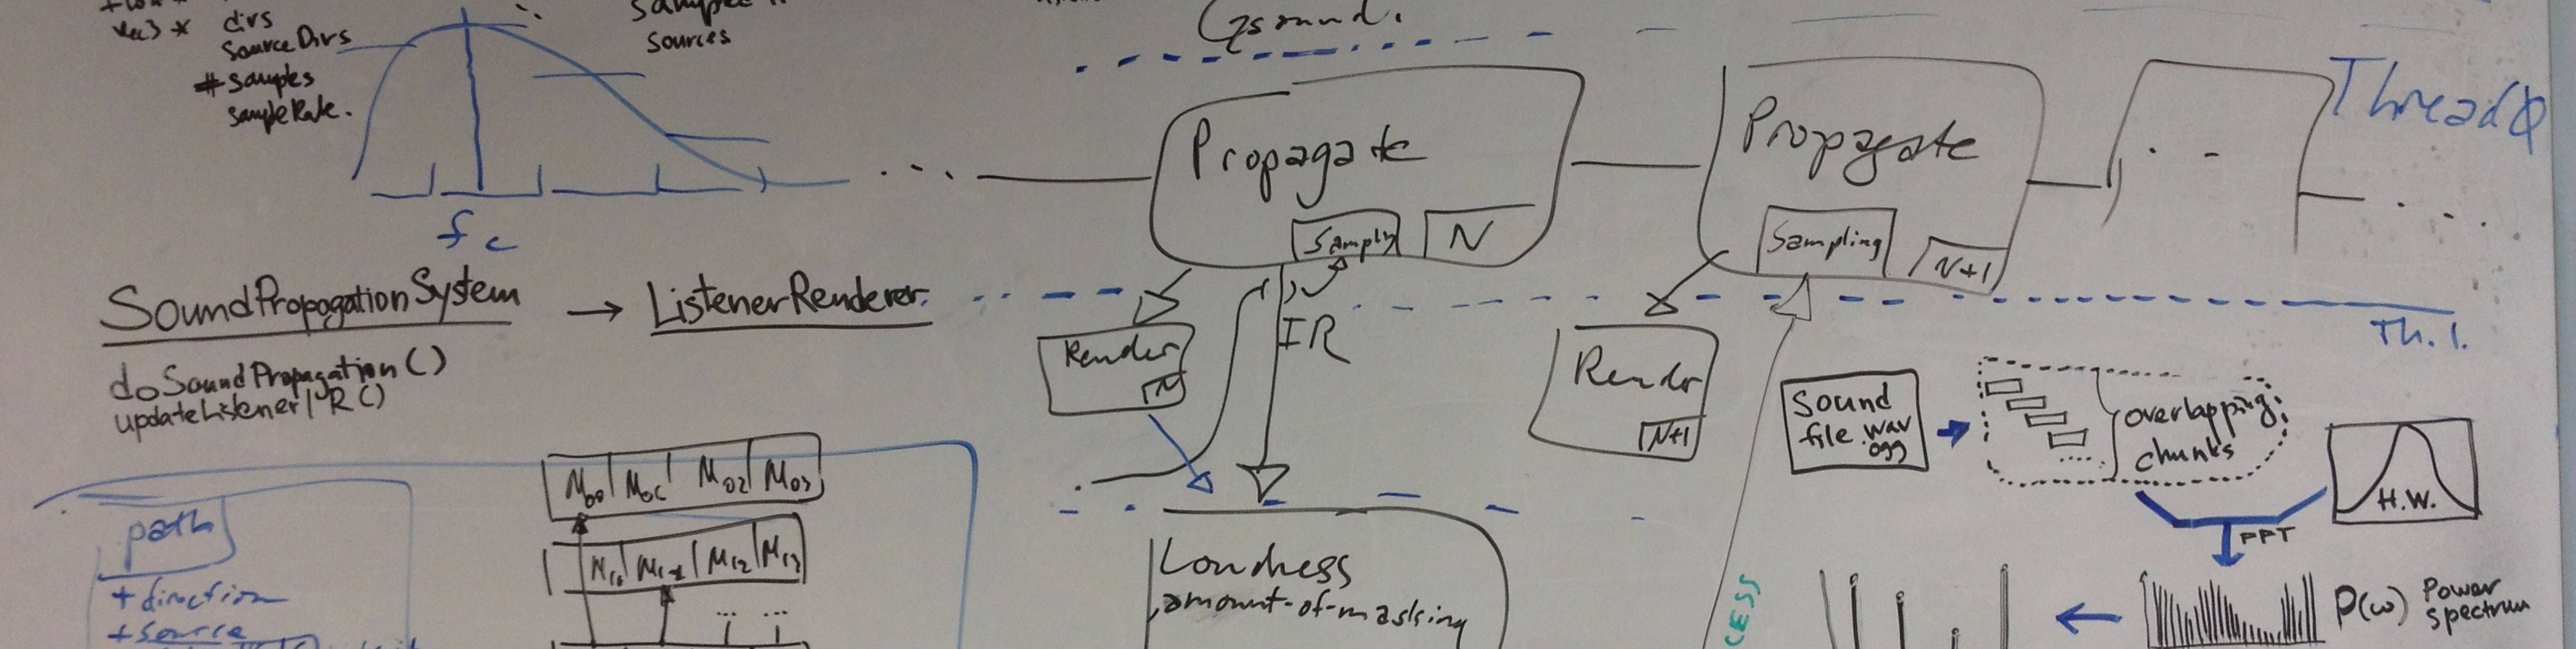
\includegraphics[height=1.5in]{figs/teaser}
   \caption{The System Design.}
 }

\maketitle

\begin{abstract}

\begin{abstract}
Your abstract goes here...
\end{abstract}

\end{abstract}

\begin{CRcatlist}
  \CRcat{I.3.5}{Computer Graphics}{Computational Geometry and Object Modeling}{Physically based modeling}
  \CRcat{I.3.5}{Computer Graphics}{Applications}{Sound rendering};
\end{CRcatlist}

\keywordlist

%% Required for all content. 

\copyrightspace


\section{Introduction}
[intro]

\newpage
\section{Related Work}
Our work is based on ray-tracing methods of sound propagation simulation, and psychoacoustic principles of human auditory system. In this section we give brief overview of related work in geometric sound propagation, perceptual coding, and perceptual audio rendering.

\paragraph{Geometric Sound Propagation} 

%[Sound Simulation pipeline overview? short: synthesis, propagation and rendering (diagram).]

There are two main approaches in solving the problem of sound propagation: wave-based \cite{savioja2010real,thompson2006review,gumerov2009wideband} and geometric \cite{funkhouser2003survey}, with an accuracy and computational complexity being the major trade-offs between them. In wave-based approach the acoustic wave equation being solved numerically, while in geometric approach the problem is reduced to geometric computations assuming the rectilinear propagation of sound waves. Due to the high computational demands of wave-based methods, the field of interactive sound propagation algorithms is primarily dominated by geometric methods, although there are interactive wave-based methods for static scenes \cite{raghuvanshi2010precomputed,mehra2013wave}.

Geometric approach includes algorithms based on image source \cite{borish1984extension}, beam tracing \cite{tsingos2001modeling}, frustum tracing \cite{chandak2009fastv}, ray tracing \cite{taylor2012guided,schissler2014high}. Recent advances in ray tracing based approach together with its highly parallel nature makes it stand out among other geometric approachers for interactive sound simulation applications \cite{taylor2010sound,schissler2011gsound}. The general idea behind ray tracing based algorithms is to model sound propagation effect by considering different paths between a source and a listener. These propagation paths encode information about the delays and attenuations of sound traveling along the paths, and may consist of any number of reflections and diffractions. 

See \cite{hulusic2012acoustic} for a more comprehensive survey on acoustic rendering and auditory.

\paragraph{Psychoacoustics}

When sound wave reaches the human ear the mechanical energy is transformed into a neural signal by the basilar membrane, which eventually travels to the brain. This suggests that taking into account the perceptual transformations due to the pathway of the ear and brain may be advantageous for some sound processing applications.

The field of psychoacoustics has made significant progress toward characterizing the time-frequency analysis capabilities of the inner ear \cite{painter2000perceptual}. One notable example of applying psychoacoustic principles to digital signal processing is the perceptual coding of audio. It exploits the human auditory system's inability to hear quantization noise under the condition of auditory masking \cite{pan1995tutorial} to perform perceptually lossless audio signal compression \cite{ambikairajah1997auditory}. Models such as this have been successfully applied to different audio compression formats, including MPEG-1 Audio Layer III (MP3).

The main psychoacoustic principles consist of absolute hearing thresholds, critical band frequency analysis, simultaneous masking, the spread of masking, and temporal masking. Making use of these psychoacoustic notions in the audio simulation system allows ...  

% Combining these psychoacoustic notions with basic properties of signal quantization has also led to the theory of perceptual entropy [45], a quantitative estimate of the fundamental limit of transparent audio signal compression.

% Perceptual methods, e.g. perceptually based rendering, have been used in computer graphics research.

\paragraph{Perceptual Audio Rendering} 

Our work is related to the work of \cite{tsingos2004perceptual}, where the psychoacoustic principles are utilized to handle large number of sources and accelerate sound rendering.
Similar approach was done in \cite{moeck2007progressive} for producing scalable or progressive rendering of complex mixtures of sounds.
Our work differs from the previous two in that we intend to leverage psychoacoustic feedback throughout the entire pipeline (including propagation), not only in rendering phase or for clustering.

% Many techniques have been proposed in the literature to handle multiple sources: sound source clustering [Tsingos et al. 2004], and a combination of hierarchical clustering and perceptual metrics [Moeck et al. 2007], etc. to handle a large number of sources.
% Perceptual techniques [Moeck et al. 2007] to handle large number of sources and accelerate sound rendering.
% All the interactive geometric propagation algorithms can handle only small number of sound sources. Perceptual ... (Tsingos) can help increase the number of sources by clustering them based on...



\section{The Psychoacoustic Model}
%\paragraph{Intro}
Psychoacoustics is the science of auditory perception and the human experience of hearing.
Limitations induced by the psychological and physiological mechanisms responsible for hearing are of particular 
interest and have been successfully applied to musical composition, architecture, digital audio coding, and mixing/rendering 
sound.
%and in particular the limitations induced by the psychological and physiological
%mechanisms responsible for the experience of hearing.
Individual psychoacoustic effects and illusions are refered to as \emph{psychoacoustic principles} and include:

\begin{itemize}
\item The Absolute Threshold of Hearing
\item Critical Band Frequency Analysis
\item Simultaneous Masking
\item Non-Simultaneous Masking
\item The Spread of Masking
\end{itemize}

In this method we seek to demonstrate how these basic psychoacoustic principles can be leveraged in a geometric sound propagation 
pipeline, with our most novel contribution being the use of masking in the propagation phase of sound simulation.

\paragraph{Auditory Filters and the Bark Scale of Critical Bandwidths}
%The frequency of sound is conventionally measured in hertz but alternative scales based on human perception are more commonly used
%in psychoacoustic literature and models.
%These include the Bark and ERB frequency scales, both of which are based on the frequency resolution of human hearing and are derived 
%from listening experiments.
%Although sound frequency is conventionally measured in hertz, for the purpose of psychoacoustic modelling it is preferable to use a 
%scale based on the frequency resolution of human hearing.
%The most common scale used in psychoacoustic literature is the Bark scale, which has units directly proportional to the frequency-dependent 
%bandwidth at which individual tones can be perceived separately.
%The Bark scale is measured in \textbf{critical bands}, 
%Frequency scales based on the resolution of human hearing are used for modelling psychoacoustic principles, most commonly the Bark scale.
%The Bark scale is measured in units of \emph{critical bands}

The perception of sound frequency is mediated by the \textbf{basilar membrane}, a coiled structure of the inner ear that vibrates in response 
to sound energy.
Regions of the basilar membrane have a characteristic frequency they are most sensitive to. This characteristic frequency is highest at the 
base of the basilar membrane and continuously decreases along it's length.
Pure tones result in patterns of excitation on the basilar membrane that may overlap for sounds that are nearby in frequency, and for this reason the 
basilar membrane is abstracted in literature as a bank of overlapping \textbf{auditory filters}.
%The bandwidth of an auditory filter is referred to as it's \textbf{critical bandwidth}
\textbf{The Bark frequency scale} is measured in units of the frequency-dependent bandwidths of the auditory filters of the basilar membrane, refered 
to as the \textbf{critical bandwidths}, and is a commonly used frequency scale in psychoacoustics because it is directly proportional to the frequency 
resolution of human hearing.
%whose bandwidths are measured by \textbf{the Bark scale}.
%Both the Bark scale and the curves representing auditory filters along the basilar membrane have been derived from listening experiments.
%The shape of these auditory filters have been derived from listening experiments and used to design a frequency scale proportional to the 
%frequency resolution of human hearing
%, and this overlap 
%has been measured through listening experiments.


\begin{figure}
  \centerline{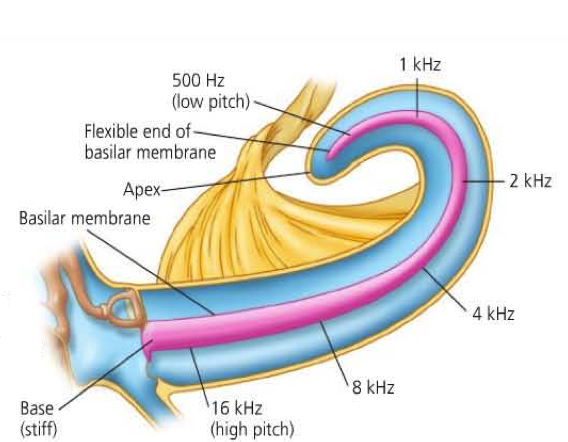
\includegraphics[width=2.8in]{figs/bmem}}
  \caption{The basilar membrane}
  \label{fig:basilarmembrane}
\end{figure}

%The basilar membrane is the auditory equivalent of the human eyes.
%It mediates human auditory perception as well as the phenomenon of spectral masking.
%The following is a brief overview of it's function as it relates to psychoacoustic principles.


\section{Overview}

\subsection{Spectral Masking}
[spectral masking]


\subsection{GSound}
\input{gsound.tex



%\section{Conclusions}
%[conclusions]


\section{Conclusion and Outlook} % instead of limitations and future works
% \paragraph{Limitations}

% \paragraph{Conclusion}

% \paragraph{Future Work}

\begin{itemize}
\item Incorporate temporal masking by filtering the masking thresholds computed from the IR

\item Incorporate HRTFs in the calculation of directional excitation
% Incorporate bidirectional ray tracing instead of backwards ray tracing of the sound paths.

\item Try strategies to connect the paths and guide sampling on both ends to converge more efficiently

\item Improve sampling schemes based on the state-of-the-art multiple importance sampling algorithms from light transport

\item Binaural masking.

\item Use psychoacoustic metrics to mutate existing paths for manifold exploration

\item Go deeper into Rendering part of the system (how can we use psychoacoustic principles there)

\end{itemize}



% \begin{table}[ht]
%   \centering
%   \caption{A simple table.}
%   \begin{tabular}{|r|l|}
%     \hline
%     7C0 & hexadecimal \\
%     3700 & octal \\ \cline{2-2}
%     11111000000 & binary \\
%     \hline \hline
%     1984 & decimal \\
%     \hline
%   \end{tabular}
% \end{table}


% The SIGGRAPH citation format is the ``author year''
% format~\cite{Pellacini:2005:LAH}. The year is separated from the
% author by a single space~\cite{yee:2000:ssa}. Two authors are
% separated by the word ``and''~\cite{parke:1996:CFA}. More than two
% authors are represented by the primary author and ``et al.''~\cite{levoy:2000:TDM}.

% Multiple citations at a single point in the content are separated by
% semicolons~\cite{levoy:2000:TDM,sako:2001:SSB}.

% When the last name of the cited author is part of the text, it may be
% omitted from the citation: ``\ldots as shown in Fedkiw et
% al.~\shortcite{fedkiw:2001:VSO}, the coefficient remains\ldots''


% Shown in Figure~\ref{fig:ferrari}.

% \begin{figure}[ht]
%   \centering
%   \includegraphics[width=3.0in]{images/ferrari_laferrari}
%   \caption{Ferrari LaFerrari. Image courtesy Flickr user ``gfreeman23.''}
%   \label{fig:ferrari}
% \end{figure}

%\section{Contact Information}
%
%If you have questions or suggestions regarding this document, please
%contact us at ``gamma@cs.unc.edu''.

\section*{Acknowledgements}

To Celeste, for the pizza and coffee, and Hasan, for all the bagels.

\bibliographystyle{acmsiggraph}
\nocite{*}
\bibliography{src/references}
\end{document}
